\documentclass[12pt,a4paper,twocolumn]{article}
% The following LaTeX packages must be installed on your machine: amsmath, authblk, bm, booktabs, caption, dcolumn, fancyhdr, geometry, graphicx, hyperref, latexsym, natbib
\input{151.dat}
\usepackage{gensymb}
\usepackage{amsthm}
\usepackage{float}
\usepackage{siunitx}
\usepackage{amssymb}
\usepackage{float}
\usepackage{enumerate}
\usepackage{listings}
\usepackage{mathtools}
\PassOptionsToPackage{hyphens}{url}\usepackage{hyperref}
\usepackage[none]{hyphenat}
\usepackage{physics}
\newcommand\ddfrac[2]{\frac{\displaystyle #1}{\displaystyle #2}}
%\renewcommand{\familydefault}{\sfdefault}


\begin{document}

\setcounter{page}{1}

\section*{PS 49: Problem 4.29}
\bigskip

\begin{enumerate}[(a)]

\item

\item Letting the program run with parameters $d = 3$, $N = 40$, and $E = 40$ for a time $> 100,000$ mcs, we obtain the mean energy of the demon $\ev{E_d} = 0.65$, and the mean energy per particle $\ev{E}/N = 0.98$. For varying $N$, we have the following:

\begin{table}[h!]
	\centering
	\caption{Energy values for $E = 40$.}
	\begin{tabular}{|c|c|c|c|}
		\hline
		$N$ & $\ev{E_d}$ & $\ev{E}$ & $\ev{E}/N$ \\ \hline
		40 & 0.65 & 39.35 & 0.984 \\
		60 & 0.438 & 0.329 & 0.659 \\
		80 & 0.329 & 39.671 & 0.496 \\
		100 & 0.265 & 39.735 & 0.397 \\ \hline
	\end{tabular}
	\label{tab:E=40}
\end{table}

\begin{figure}[h!]
	\centering
	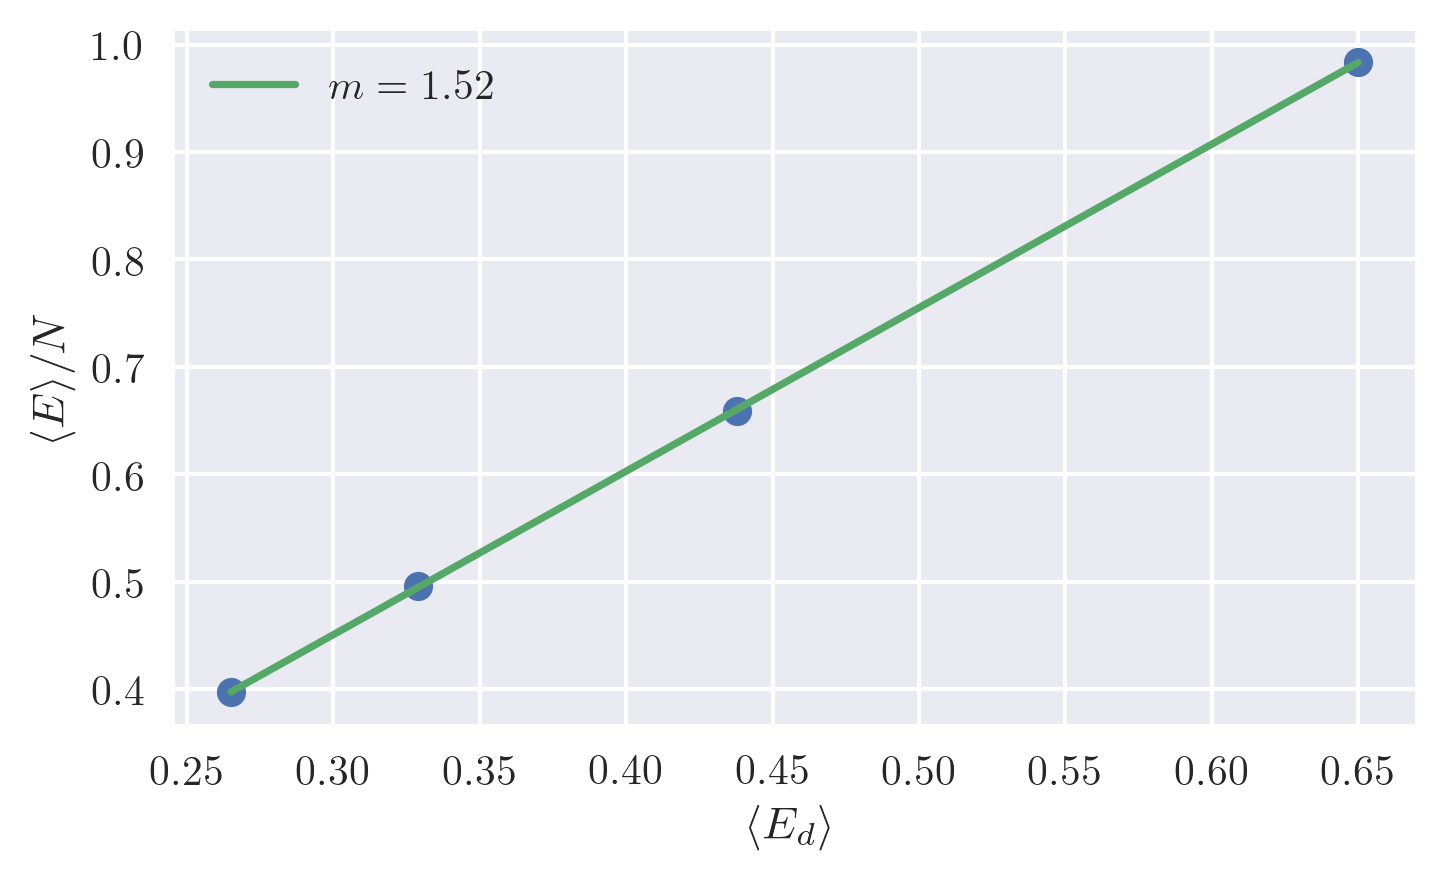
\includegraphics[width=\linewidth]{E=40.png}
	\caption{Relationship between $\ev{E_d}$ and $\ev{E}/N$ for $N=40$.}
	\label{fig:E=40}
\end{figure}

From linear regression, we observe a direct relationship between $\ev{E_d}$ and $\ev{E}/N$, with a proportionality constant $m = 1.52$ or $m = \frac{31}{20} \approx \frac{3}{2}$. This implies the relation

\begin{equation}
	\boxed{
		\frac{\ev{E}}{N} \approx \frac{3}{2} \ev{E_d}
	} \label{eq:answer-b}
\end{equation}

\item The mean energy of an ideal classical gas is 3 dimensions is

\begin{equation}
	\ev{E} = \frac{3}{2}NkT \label{eq:energy-ideal}
\end{equation}

Setting units of $k = 1$, and rearranging terms,

\begin{equation}
	\frac{\ev{E}}{N} = \frac{3}{2}T \label{eq:energy-unity}
\end{equation}

But \eqref{eq:answer-b} implies

\begin{equation}
	\frac{3}{2}\ev{E_d} = \frac{3}{2}T
\end{equation}

or

\begin{equation}
	\boxed{
		\ev{E_d} = T
	} \label{eq:answer-c}
\end{equation}

which means that the temperature of the gas is equal to the mean energy of the demon at any $N$.


\end{enumerate}

\end{document}